\documentclass{standalone}
\usepackage[dvipsnames]{xcolor}
\usepackage{tikz}
%\usepackage{pgfplots}
%\usepackage{pgfplotstable}
%\pgfplotsset{compat=1.5}

\tikzstyle{v par}=              [dash pattern=on 10pt off 5pt,color=red,line width = 2pt]
\tikzstyle{z direction}=      [dash pattern=on 10pt off 5pt on 2pt off 5pt, color=Blue,line width = 2pt]

\begin{document}
{
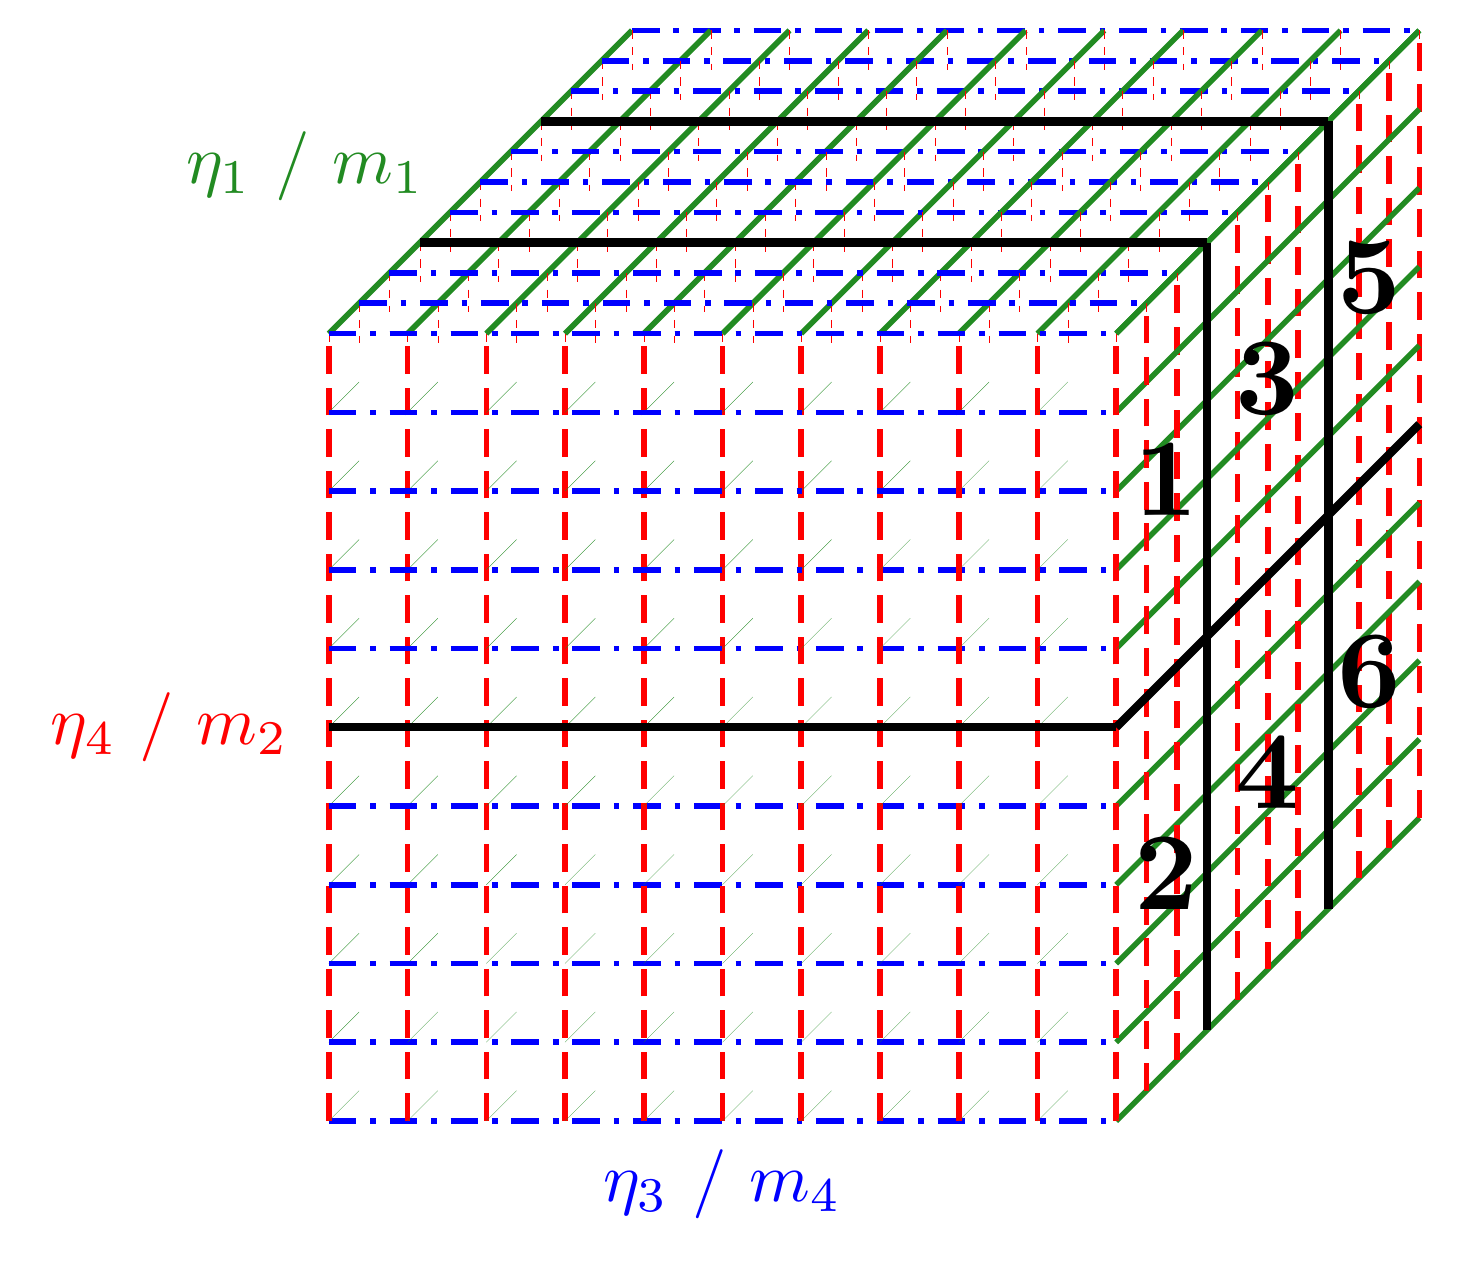
\begin{tikzpicture}
\def\n{10}
\foreach \x in{0,...,\n}
{   \draw[z direction] (0,\x ,\n) -- (\n,\x ,\n);
    \draw[v par] (\x ,0,\n) -- (\x ,\n,\n);
    \draw[ForestGreen,line width=2pt] (\n,\x ,\n) -- (\n,\x ,0);
    \draw[ForestGreen,line width=2pt] (\x ,\n,\n) -- (\x ,\n,0);
    \draw[v par] (\n,0,\x ) -- (\n,\n,\x );
    \draw[z direction] (0,\n,\x ) -- (\n,\n,\x );
    \foreach \y in {0,...,\n}
     {
      \draw[ForestGreen,line width=0.1pt] (\x,\y,\n) -- (\x,\y,\n-1);
      \draw[red,dashed,line width=0.1pt] (\x,\n,\y) -- (\x,\n-0.5,\y);
      %\draw[Blue,line width=0.1pt] (\n,\x,\y) -- (\n-0.5,\x,\y);
     }
}
\node[scale=2.5,Blue] at (\n/2,-.8,\n) {$\eta_3$ / $m_4$};
\node[scale=2.5,red,left] at (-.2,\n/2,\n) {$\eta_4$ / $m_2$};
\node[scale=2.5,ForestGreen,left] at (-0.4,\n+0.2,\n/2) {$\eta_1$ / $m_1$};

\draw[line width=3pt] (0,5,\n) -- (\n,5,\n);
\draw[line width=3pt] (\n,5,0) -- (\n,5,\n);
\draw[line width=3pt] (0,\n,3) -- (\n,\n,3);
\draw[line width=3pt] (\n,0,3) -- (\n,\n,3);
\draw[line width=3pt] (0,\n,7) -- (\n,\n,7);
\draw[line width=3pt] (\n,0,7) -- (\n,\n,7);

\node[scale=4] at (\n,\n*3/4,\n*5/6) {\bf 1};
\node[scale=4] at (\n,\n*3/4,\n*3/6) {\bf 3};
\node[scale=4] at (\n,\n*3/4,\n/6) {\bf 5};
\node[scale=4] at (\n,\n/4,\n*5/6) {\bf 2};
\node[scale=4] at (\n,\n/4,\n*3/6) {\bf 4};
\node[scale=4] at (\n,\n/4,\n/6) {\bf 6};

\end{tikzpicture}
}
\end{document}